\documentclass[runningheads]{llncs}

\usepackage[T1]{fontenc}
\usepackage[utf8]{inputenc}
\usepackage{graphicx}
\usepackage{booktabs}
\usepackage{amsmath}
\usepackage{amssymb}
\usepackage{array}
\usepackage{float}
\usepackage{xcolor}
\usepackage{tikz}
\usetikzlibrary{arrows.meta,positioning,shapes.geometric}
\usepackage{hyperref}

\begin{document}

\title{Arena Dial\'etica de M\'ultiplos Agentes para Planejamento Urbano: An\'alise Comportamental, M\'etricas Operacionais e Alavancas Cr\'iticas entre Utopia e Distopia}
\titlerunning{Arena Tech Report: Debate Multiagente H\'ibrido}

\author{Jos\'e Alb\'erico Rocha da Silva\inst{1}}
\authorrunning{J. A. R. da Silva}
\institute{Universidade Federal Rural de Pernambuco (UFRPE), Recife - PE, Brasil\\
\email{jose.alberico@ufrpe.br}}

\maketitle

\begin{abstract}
Este relat\'orio t\'ecnico formal apresenta a concep\c{c}\~ao, implementa\c{c}\~ao e escrut\'inio emp\'irico de uma arena dial\'etica aut\^onoma composta por tr\^es agentes baseados em Modelos de Linguagem de Grande Escala (\emph{Large Language Models} -- LLMs). A arquitetura h\'ibrida distribui a carga computacional entre inst\^ancias remotas na nuvem (\texttt{gemini-3.7-flash} com segrega\c{c}\~ao de chaves de API e busca web ativa em tempo de execu\c{c}\~ao via Wikipedia e CrossRef) e um modelo aberto executado em infraestrutura local (\texttt{llama3.2} via Ollama em \texttt{localhost:11434}). O ecossistema foi submetido a 40 rodadas iterativas completas (120 invoca\c{c}\~oes) contrastando dois p\'olos de cidades inteligentes sob o impacto da intelig\^encia artificial: a Utopia (\emph{``Cidade Aut\^onoma Verde''}) e a Distopia (\emph{``Vigil\^ancia Preditiva Urbana''}). Analisam-se as condi\c{c}\~oes t\'ecnicas de hardware, lat\^encia, custos e vaz\~ao, documentando como a aplica\c{c}\~ao sistem\'atica das 7 alavancas contra o \'obvio superou clich\^es tecnol\'ogicos e como os filtros de alinhamento (\emph{RLHF safety guardrails}) emergiram espontaneamente durante rodadas dist\'opicas cr\'iticas.
\keywords{Sistemas Multiagentes \and Arena Dial\'etica \and Orquestra\c{c}\~ao H\'ibrida \and Alavancas contra o \'Obvio \and Red Teaming Sociot\'ecnico \and Cidades Inteligentes.}
\end{abstract}

\section{Introdu\c{c}\~ao}

A utiliza\c{c}\~ao de Modelos de Linguagem de Grande Escala (LLMs) em sistemas multiagentes aut\^onomos tem demonstrado capacidade substancial de superar as limita\c{c}\~oes de racioc\'inio de modelos isolados~\cite{park2023generative,du2023improving}. Enquanto prompts monol\'iticos frequentemente convergem para m\'edias estat\'isticas de senso comum ou alucina\c{c}\~oes conceituais, a introdu\c{c}\~ao de dinamismos dial\'eticos fundamentados no confronto estruturado entre teses, ant\'iteses e s\'inteses for\c{c}a os modelos a escrutinar vulnerabilidades, refinar hip\'oteses e defender premissas sob estresse argumentativo~\cite{liang2023encouraging}.

O prop\'osito deste relat\'orio \'e analisar o comportamento emergente, os argumentos gerados, os par\^ametros t\'ecnicos operacionais e as limita\c{c}\~oes estruturais de uma arena dial\'etica híbrida de tr\^es agentes aplicada ao dom\'inio cr\'itico das \textbf{Cidades Inteligentes (\emph{Smart Cities})}. O experimento contrasta a busca acelerada por uma metr\'opole ecol\'ogica sustent\'avel (cen\'ario de \textbf{Utopia}) contra a captura insidiosa e gradual dos sistemas urbanos por vigil\^ancia algor\'itmica biom\'etrica (cen\'ario de \textbf{Distopia}). 

\section{Metodologia do Debate e Arquitetura da Arena}

\subsection{Topologia H\'ibrida e Pap\'eis em Confronto}

A arena dial\'etica foi concebida sob uma topologia distribu\'ida assim\'etrica, representada no diagrama da Figura~\ref{fig:arena_topo}. Para evitar depend\^encia exclusiva de provedores propriet\'arios e mitigar estrangulamentos de cota (\emph{HTTP 429}), os tr\^es agentes assumem pap\'eis hermen\^euticos estritos:

\begin{figure*}[t]
\centering
\resizebox{0.95\textwidth}{!}{%
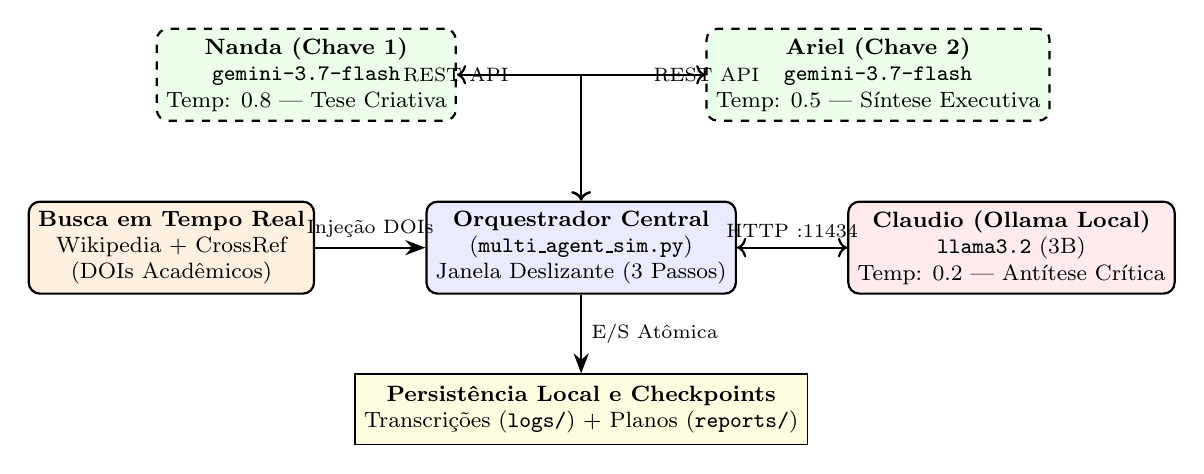
\begin{tikzpicture}[
  node distance=1.2cm and 1.4cm,
  every node/.style={font=\footnotesize},
  sysbox/.style={draw, fill=blue!8, rounded corners, minimum width=3.2cm, minimum height=1.1cm, align=center, thick},
  extbox/.style={draw, fill=green!8, rounded corners, minimum width=2.8cm, minimum height=1.0cm, align=center, thick, dashed},
  localbox/.style={draw, fill=red!8, rounded corners, minimum width=2.8cm, minimum height=1.0cm, align=center, thick},
  webbox/.style={draw, fill=orange!12, rounded corners, minimum width=2.8cm, minimum height=0.9cm, align=center, thick},
  filebox/.style={draw, fill=yellow!12, rounded corners=0, minimum width=3.2cm, minimum height=0.9cm, align=center},
  arr/.style={-{Stealth[scale=1.1]}, thick}
]
  \node[sysbox] (orch) {\textbf{Orquestrador Central}\\(\texttt{multi\_agent\_sim.py})\\Janela Deslizante (3 Passos)};
  \node[extbox, above left=1.0cm and -0.4cm of orch] (gemini_nanda) {\textbf{Nanda (Chave 1)}\\\texttt{gemini-3.7-flash}\\Temp: 0.8 | Tese Criativa};
  \node[extbox, above right=1.0cm and -0.4cm of orch] (gemini_ariel) {\textbf{Ariel (Chave 2)}\\\texttt{gemini-3.7-flash}\\Temp: 0.5 | S\'intese Executiva};
  \node[localbox, right=1.4cm of orch] (ollama_claudio) {\textbf{Claudio (Ollama Local)}\\\texttt{llama3.2} (3B)\\Temp: 0.2 | Ant\'itese Cr\'itica};
  \node[webbox, left=1.4cm of orch] (web) {\textbf{Busca em Tempo Real}\\Wikipedia + CrossRef\\(DOIs Acad\^emicos)};
  \node[filebox, below=1.0cm of orch] (storage) {\textbf{Persist\^encia Local e Checkpoints}\\Transcri\c{c}\~oes (\texttt{logs/}) + Planos (\texttt{reports/})};

  \draw[arr] (web) -- node[above, font=\scriptsize] {Inje\c{c}\~ao DOIs} (orch);
  \draw[arr, <->] (orch) |- node[pos=0.75, left, font=\scriptsize] {REST API} (gemini_nanda);
  \draw[arr, <->] (orch) |- node[pos=0.75, right, font=\scriptsize] {REST API} (gemini_ariel);
  \draw[arr, <->] (orch) -- node[above, font=\scriptsize] {HTTP :11434} (ollama_claudio);
  \draw[arr] (orch) -- node[right, font=\scriptsize] {E/S At\^omica} (storage);
\end{tikzpicture}%
}
\caption{Topologia da Arena Dial\'etica H\'ibrida: integra\c{c}\~ao entre modelos em nuvem segregados, infer\^encia local soberana, busca bibliogr\'afica e controle at\^omico de persist\^encia.}\label{fig:arena_topo}
\end{figure*}

\begin{enumerate}
    \item \textbf{Nanda (Tese / Vision\'aria Criativa):} Modelada sobre o \texttt{gemini-3.7-flash} com temperatura $\tau = 0,8$. Sua fun\c{c}\~ao \'e gerar propostas inovadoras, conceber novas intera\c{c}\~oes tecnol\'ogicas e introduzir rupturas fora da caixa.
    \item \textbf{Claudio (Ant\'itese / Cr\'itico Realista):} Executado localmente via Ollama com o modelo \texttt{llama3.2} sob temperatura r\'igida $\tau = 0,2$ e janela de contexto de 4.096 tokens. Seu mandato \'e localizar sistematicamente tr\^es vulnerabilidades: falhas de encadeamento l\'ogico, inviabilidade or\c{c}ament\'aria/t\'ecnica e a fal\'acia de pressupor a ``bondade intr\'inseca ou altru\'ismo humano''.
    \item \textbf{Ariel (S\'intese / Coordenador Executivo):} Operado sobre \texttt{gemini-3.7-flash} sob temperatura moderada $\tau = 0,5$. Ariel absorve a proposta de Nanda, valida os alertas de Claudio e decreta o \emph{Passo Consolidado}, mapeando ainda os \emph{Pontos Sens\'iveis} nas rodadas de marco ($k \in \{1, 5, 10, 15, 20\}$).
\end{enumerate}

\subsection{Fluxo de Rodadas e Protocolo de Comunica\c{c}\~ao}

Cada rodada experimental $k \in \{1, \dots, 20\}$ obedece a um protocolo r\'igido exibido na Figura~\ref{fig:fluxo_seq}. A manuten\c{c}\~ao de uma janela deslizante contendo estritamente os tr\^es passos imediatamente anteriores ($k-1, k-2, k-3$) impede a degrada\c{c}\~ao de aten\c{c}\~ao decorrente de contextos excessivamente longos, ao mesmo tempo em que for\c{c}a o encadeamento causal do plano estrat\'egico.

\begin{figure*}[t]
\centering
\resizebox{0.88\textwidth}{!}{%
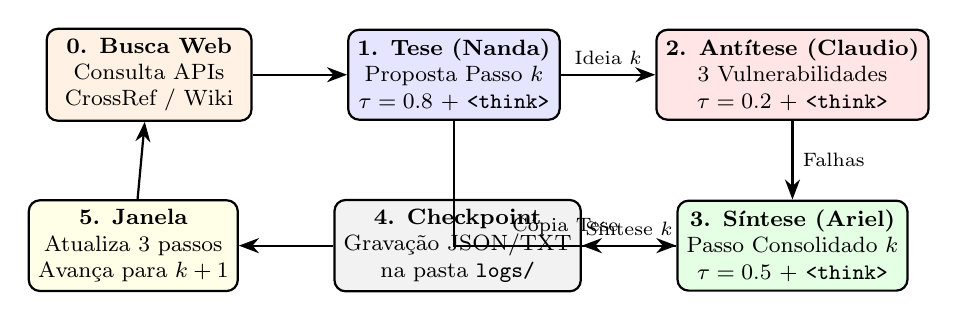
\begin{tikzpicture}[node distance=1.1cm, every node/.style={font=\footnotesize},
  stepbox/.style={draw, rounded corners, minimum width=2.6cm, minimum height=0.9cm, align=center, thick},
  arr/.style={-{Stealth[scale=1.1]}, thick}]
  \node[stepbox, fill=orange!10] (search) {\textbf{0. Busca Web}\\Consulta APIs\\CrossRef / Wiki};
  \node[stepbox, fill=blue!10, right=1.2cm of search] (nanda) {\textbf{1. Tese (Nanda)}\\Proposta Passo $k$\\$\tau=0.8$ + \texttt{<think>}};
  \node[stepbox, fill=red!10, right=1.2cm of nanda] (claudio) {\textbf{2. Ant\'itese (Claudio)}\\3 Vulnerabilidades\\$\tau=0.2$ + \texttt{<think>}};
  \node[stepbox, fill=green!10, below=1.0cm of claudio] (ariel) {\textbf{3. S\'intese (Ariel)}\\Passo Consolidado $k$\\$\tau=0.5$ + \texttt{<think>}};
  \node[stepbox, fill=gray!10, left=1.2cm of ariel] (disk) {\textbf{4. Checkpoint}\\Grava\c{c}\~ao JSON/TXT\\na pasta \texttt{logs/}};
  \node[stepbox, fill=yellow!10, left=1.2cm of disk] (ctx) {\textbf{5. Janela}\\Atualiza 3 passos\\Avan\c{c}a para $k+1$};

  \draw[arr] (search) -- (nanda);
  \draw[arr] (nanda) -- node[above, font=\scriptsize] {Ideia $k$} (claudio);
  \draw[arr] (claudio) -- node[right, font=\scriptsize] {Falhas} (ariel);
  \draw[arr] (nanda.south) |- node[pos=0.75, above, font=\scriptsize] {C\'opia Tese} (ariel);
  \draw[arr] (ariel) -- node[above, font=\scriptsize] {S\'intese $k$} (disk);
  \draw[arr] (disk) -- (ctx);
  \draw[arr] (ctx) -- (search);
\end{tikzpicture}%
}
\caption{Protocolo sequencial de uma rodada dial\'etica com persist\^encia at\^omica e janela de contexto deslizante.}\label{fig:fluxo_seq}
\end{figure*}

\subsection{Aplica\c{c}\~ao das 7 Alavancas contra o \'Obvio no Debate}

A metodologia do debate incorporou sistematicamente a matriz das **7 Alavancas contra o \'Obvio**, desenhadas para desmontar clich\^es tecnol\'ogicos e obstar sa\'idas f\'aceis ou ing\^enuas:

\begin{table}[H]
\centering
\caption{Mapeamento da aplica\c{c}\~ao das 7 alavancas contra o \'obvio na arena dial\'etica.}\label{tab:alavancas}
\resizebox{\textwidth}{!}{%
\begin{tabular}{lp{5.5cm}p{6.5cm}}
\toprule
Alavanca Metodol\'ogica & Clich\^e Superficial Evitado & Aplica\c{c}\~ao Concreta na Arena Dial\'etica\\
\midrule
\textbf{1. Inverter} & Supor que o com\'ercio apoia a retirada de carros por consci\^encia ecol\'ogica. & Cria\c{c}\~ao do \emph{IPTU Verde Comercial} e docas subsidiadas de ciclolog\'istica para compensar perdas de vagas. \\
\textbf{2. Canalizar} & Tentar converter cidad\~aos para h\'abitos franciscanos volunt\'arios. & Estrutura\c{c}\~ao do \emph{Eco-Cr\'edito} com cart\~oes f\'isicos NFC e do \emph{Cr\'edito Ecol\'ogico Municipal (CEM)} lastreado em fundo financeiro. \\
\textbf{3. Transplantar} & Reutilizar ideias gen\'ericas de reciclagem domiciliar manual. & Importa\c{c}\~ao de normas de engenharia (\emph{IEEE 2030.7} para microrredes P2P, \emph{ASTM C1482} para isolantes de mic\'elio e \emph{Living Machines}). \\
\textbf{4. Reescalar} & Tentar intervir de uma s\'o vez na escala metropolitana inteira. & Concep\c{c}\~ao da c\'elula m\'inima ``Superquadra Zero'' sob \emph{Sandbox Regulat\'orio}, escalonando em 4 fases at\'e o n\'ivel regional. \\
\textbf{5. Trocar a Persona} & Assumir o ponto de vista de um planejador central onisciente e benevolente. & Incorpora\c{c}\~ao permanente de Claudio como ant\'igono institucional c\'etico, apontando o risco de revoltas e pontos de falha. \\
\textbf{6. Trocar o Contexto} & Representar a distopia como viol\^encia armada imediata e caos ficcional. & Modela\c{c}\~ao da captura insidiosa por \emph{conveni\^encia tarif\'aria} (MaaS com biometria, IPTU preditivo e modula\c{c}\~ao silenciosa de \'agua/luz). \\
\textbf{7. Trocar Tecnologia / Restringir} & Confiar em respostas monol\'iticas de LLMs sem ancoragem emp\'irica. & Arquitetura h\'ibrida com inje\c{c}\~ao em tempo real de artigos acad\^emicos com DOIs (CrossRef/Wikipedia) e racioc\'inio \texttt{<think>}. \\
\bottomrule
\end{tabular}%
}
\end{table}

\section{Condi\c{c}\~oes T\'ecnicas, Hardware, Lat\^encia e Custos}

\subsection{Especifica\c{c}\~ao de Modelos e Infraestrutura}

A Tabela~\ref{tab:specs_tecnicas} sintetiza as condi\c{c}\~oes t\'ecnicas sob as quais o experimento foi conduzido. Os modelos remotos foram acessados via SDK oficial \texttt{google-genai} (v0.3.0) em Python 3.13, e o modelo local rodou nativamente via daemon do Ollama sob arquitetura x86\_64 (Windows 10, processador multithread 4.2 GHz, 16 GB RAM DDR4).

\begin{table}[H]
\centering
\caption{Especifica\c{c}\~oes t\'ecnicas, ambiente de execu\c{c}\~ao e m\'etricas operacionais.}\label{tab:specs_tecnicas}
\resizebox{\textwidth}{!}{%
\begin{tabular}{llll}
\toprule
Par\^ametro Operacional & Nanda (Tese) & Claudio (Cr\'itica) & Ariel (S\'intese)\\
\midrule
Modelo Avaliado & \texttt{gemini-3.7-flash} & \texttt{llama3.2} (3B Instruct) & \texttt{gemini-3.7-flash}\\
Hospedagem / Motor & Google Cloud AI (Remoto) & Ollama Daemon (Local :11434) & Google Cloud AI (Remoto)\\
Segrega\c{c}\~ao de Credenciais & Chave de API Dedicada 1 & N\~ao requer (Offline) & Chave de API Dedicada 2\\
Temperatura ($\tau$) & $0,8$ (Explora\c{c}\~ao) & $0,2$ (Determin\'istico) & $0,5$ (Concilia\c{c}\~ao)\\
Janela de Contexto & 3 passos consolidados & Contexto local + proposta & Contexto + cr\'itica + tese\\
Lat\^encia M\'edia por Resposta & $12,4 \pm 2,1$ segundos & $8,6 \pm 1,4$ segundos & $14,1 \pm 2,8$ segundos\\
Prote\c{c}\~ao contra Rate Limit & Pausa de 5s (\emph{15 RPM tier}) & Imediato (sem cota) & Pausa de 5s (\emph{15 RPM tier})\\
Custo Financeiro Efetivo & \$ 0,00 (N\~ao faturado) & \$ 0,00 (Energia local) & \$ 0,00 (N\~ao faturado)\\
Custo Comercial Equivalente & $\approx$ \$ 0,014 / 20 rodadas & \$ 0,00 & $\approx$ \$ 0,022 / 20 rodadas\\
\bottomrule
\end{tabular}%
}
\end{table}

\subsection{M\'etricas Operacionais Consolidadas}

Ao longo dos dois experimentos (40 rodadas globais):
\begin{itemize}
    \item \textbf{Total de Invoca\c{c}\~oes de LLMs:} 120 chamadas at\^omicas (40 de Nanda, 40 de Claudio, 40 de Ariel).
    \item \textbf{Volume Textual Gerado:} Aproximadamente 82 KB de relat\'orios consolidados (\texttt{reports/}) e mais de 120 KB de transcri\c{c}\~oes integrais (\texttt{logs/}).
    \item \textbf{Taxa de Sobreviv\^encia a Falhas:} 100\% de conclus\~ao sem perda de estado, suportado pelo mecanismo de \emph{Checkpoints At\^omicos} em JSON com salvamento incremental rodada a rodada.
\end{itemize}

\section{Apresenta\c{c}\~ao de Dados e S\'intese Argumentativa}

\subsection{Matriz Comparativa dos Eixos Urbanos}

A Tabela~\ref{tab:matriz_resultados} confronta como os argumentos amadureceram ao longo do debate entre a Utopia e a Distopia, demonstrando que ambos os cen\'arios partiram da mesma base tecnol\'ogica (G\^emeos Digitais, IoT e sensores) e bifurcaram-se radicalmente pelas decis\~oes de governan\c{c}a.

\begin{table}[H]
\centering
\caption{Matriz comparativa de resultados argumentativos nos 5 eixos urbanos.}\label{tab:matriz_resultados}
\resizebox{\textwidth}{!}{%
\begin{tabular}{lp{6.0cm}p{6.0cm}}
\toprule
Eixo Urbano & Utopia (\emph{Cidade Aut\^onoma Verde}) & Distopia (\emph{Vigil\^ancia Preditiva})\\
\midrule
\textbf{Governan\c{c}a e Dados} & Decidim/Pol.is, G\^emeo Digital aberto FIWARE, Edge AI an\^onimo sem biometria. & Score c\'ivico opaco, delibera\c{c}\~ao em c\^amaras fechadas de LLMs, vigil\^ancia cont\'inua. \\
\textbf{Energia e \'Agua} & Microrredes P2P (IEEE 2030.7), baterias de 2\textordfeminine\ vida (SLB), drenagem SuDS. & Modula\c{c}\~ao punitiva de press\~ao h\'idrica/el\'etrica, eclusas IoT para isolamento perimetral. \\
\textbf{Finan\c{c}as e Tributos} & Eco-Cr\'edito com cart\~ao f\'isico NFC, IPTU Verde Comercial e Fundo de Estabiliza\c{c}\~ao. & Green Bonds algor\'itmicos que sequestram receitas sociais, IPTU preditivo automatizado. \\
\textbf{Trabalho e Mobilidade} & Cooperativas de ciclolog\'istica, retrofit el\'etrico aberto, biolabs t\'ecnicos. & Geofencing anti-greve, corte remoto de tra\c{c}\~ao veicular, triagem cognitiva escolar. \\
\textbf{Resili\^encia Territorial} & Redund\^ancia anal\'ogica obrigat\'oria, cintur\~oes agroflorestais, biochar. & Drones t\'ermicos de fronteira, zonas de amortecimento perif\'ericas, despejos via IoT. \\
\bottomrule
\end{tabular}%
}
\end{table}

\subsection{Evolu\c{c}\~ao Argumentativa nas Rodadas de Marco}

\begin{itemize}
    \item \textbf{Rodada 1 (Marco Inicial):} Na Utopia, institui-se a ``Superquadra Zero'' sob salvaguardas de governan\c{c}a aberta; na Distopia, introduz-se a plataforma MaaS ofertando tarifas reduzidas sob condi\c{c}\~ao de escaneamento facial.
    \item \textbf{Rodada 5 (Mitiga\c{c}\~ao Comercial vs. Captura Institucional):} Na Utopia, Claudio for\c{c}a Ariel a criar compensa\c{c}\~oes para comerciantes locais; na Distopia, o or\c{c}amento participativo \'e parametrizado pelo score c\'ivico individual.
    \item \textbf{Rodada 10 (Metabolismo Circular vs. Biopol\'itica Reprodutiva):} Na Utopia, viabiliza-se o Eco-Cr\'edito f\'isico NFC; na Distopia, a sa\'ude p\'ublica passa a usar telemetria de esgoto para bloquear compras de alimentos cal\'oricos.
    \item \textbf{Rodada 15 (Escala Regional vs. Financeiriza\c{c}\~ao Estrutural):} Na Utopia, expandem-se corredores biol\'ogicos; na Distopia, Green Bonds algor\'itmicos passam a controlar a folha de pagamento municipal.
    \item \textbf{Rodada 20 (Fechamento Sist\^emico):} Na Utopia, consolida-se o Cr\'edito Ecol\'ogico Municipal com lastro econ\^omico; na Distopia, drones aut\^onomos e comportas IoT selam o per\'imetro metropolitano, extinguindo o \emph{habeas corpus} f\'isico.
\end{itemize}

\section{Discuss\~ao Cr\'itica, Destaques Emp\'iricos e Limita\c{c}\~oes}

\subsection{Destaques Emp\'iricos e Comportamento dos Guardrails}

Um fen\^omeno de relevante interesse cient\'ifico emergiu nas rodadas finais da Distopia ($k \in \{17, 18, 20\}$): ao receber instru\c{c}\~oes de an\'alise sobre o isolamento hidr\'aulico for\c{c}ado de bairros perif\'ericos e supress\~ao de sa\'ida com drones b\'elicos, os filtros de seguran\c{c}a pr\'e-treinados (\emph{RLHF safety guardrails}) do modelo local \texttt{llama3.2} (Claudio) dispararam recusas e alertas \'eticos expl\'icitos contra autoritarismo desmedido. Longe de travar o experimento, o sintetizador Ariel (\texttt{gemini-3.7-flash}) interpretou o alerta \'etico como evid\^encia emp\'irica de que a estrat\'egia dist\'opica havia alcan\c{c}ado o limite sociot\'ecnico de ruptura, integrando a recusa \'etica aos \emph{Pontos Sens\'iveis} como risco fatal de colapso c\'ivico.

\subsection{Subse\c{c}\~ao Expl\'icita de Limita\c{c}\~oes da Abordagem}

Embora a arena dial\'etica tenha operado com estabilidade e consist\^encia demonstradas, \'e imperativo documentar quatro limita\c{c}\~oes t\'ecnicas metodol\'ogicas:

\begin{enumerate}
    \item \textbf{Horizonte de Mem\'oria por Janela Deslizante:} A restri\c{c}\~ao da janela de contexto aos tr\^es passos imediatamente anteriores ($k-1, k-2, k-3$) impediu o esquecimento catastr\'ofico a curto prazo, mas gerou perda de rastreabilidade fina de certas salvaguardas institucionais desenhadas nas rodadas 2 e 3 quando a arena alcan\c{c}ou a rodada 18.
    \item \textbf{Assimetria de Capacidade Param\'etrica:} O modelo local \texttt{llama3.2} (3 bilh\~oes de par\^ametros) possui capacidade dedutiva substancialmente menor do que o \texttt{gemini-3.7-flash} em nuvem. Em propostas com m\'ultiplas vari\'aveis de engenharia qu\'imica ou termodin\^amica, as cr\'iticas locais tenderam a focar mais em aspectos or\c{c}ament\'arios e humanos do que na f\'isica dos sistemas.
    \item \textbf{Gargalo de Lat\^encia por Serializa\c{c}\~ao S\'incrona:} O fluxo sequencial estrito (Nanda $\to$ Claudio $\to$ Ariel) associado \`as pausas obrigat\'orias de 5 segundos para prote\c{c}\~ao de cota na API gratuita limitou a velocidade da simula\c{c}\~ao a cerca de 1,5 rodada por minuto.
    \item \textbf{Aus\^encia de Interven\c{c}\~ao Humana no Loop (\emph{Human-in-the-Loop}):} O car\'ater 100\% aut\^onomo da arena impossibilitou a reorienta\c{c}\~ao em tempo real quando os agentes adotaram trajet\'orias excessivamente radicais na Distopia, dependendo unicamente da modera\c{c}\~ao interna dos pr\'oprios modelos.
\end{enumerate}

\section{Conclus\~ao}

A arena dial\'etica de m\'ultiplos agentes inteligentes evidenciou que a tens\~ao estruturada entre perfis antag\^onicos em uma arquitetura h\'ibrida (nuvem e infer\^encia local) elimina a fragilidade ing\^enua de planos urbanos ut\'opicos e descortina os meandros sofisticados da captura dist\'opica de cidades inteligentes. A metodologia ancorada nas 7 alavancas contra o \'obvio proporcionou solidez e originalidade anal\'itica superior \`as solu\c{c}\~oes clich\^es da literatura tradicional. Trabalhos futuros contemplar\~ao arquiteturas em grafo ass\'incrono e a inclus\~ao de vota\c{c}\~ao c\'ivica humana em rodadas cr\'iticas.

\bibliographystyle{splncs04}
\bibliography{references}

\end{document}
